% Chapter 6

\chapter{Results} % Main chapter title
\section{Charged Track $v_{2}$}
Here I present measurements of elliptic flow in $\sqrt{s_{NN}}=200$ GeV d+Au collisions. Since the flattening the event plane redistributes the event plane distribution, the unidentified charged track flow can be measured directly from plots of $d\phi$. Recall that the Fourier coefficients parameterize the shape of the azimuthal hydrodynamic flow by describing it as a superposition of cosine harmonics:
\begin{equation}
\frac{d^{2}N}{dp^{2}} \propto v_0 + v_1 \cos\big(\phi - \Psi_{r}\big) + v_2 \cos\big(2(\phi - \Psi_{r})\big) + v_3 \cos\big(3(\phi - \Psi_{r})\big) \cdots
\end{equation}
where $v_0$, $v_1$, $v_2$, and $v_3$ are the values that scale the amount of spherical, directed, elliptic, and triangular flow respectively, and are indicative of collective behavior of the nuclear matter. To measure the elliptic flow we count number of tracks in bins of $d\phi$ and fit this with a function of the form:
\begin{equation}
f(x) = A [1 + B \cos 2x]
\end{equation}
where A is a term that accounts for an overall shift in the number of tracks due to statistics and B is our $v_2$. Due to the asymmetric nature of d+Au collisions, event plane calculations are significantly better on the Au going side, because of this, the following plots (figures \ref{fig:Ndphicent0}-\ref{fig:Ndphicent3}) were made using the BBC South determination of the event plane. They are binned in 5\% bins of centrality up to 15\%, at which point statistics requires the remainder of data to be binned 10\%-25\%. 

\begin{figure}[htbp!]
  \centering
    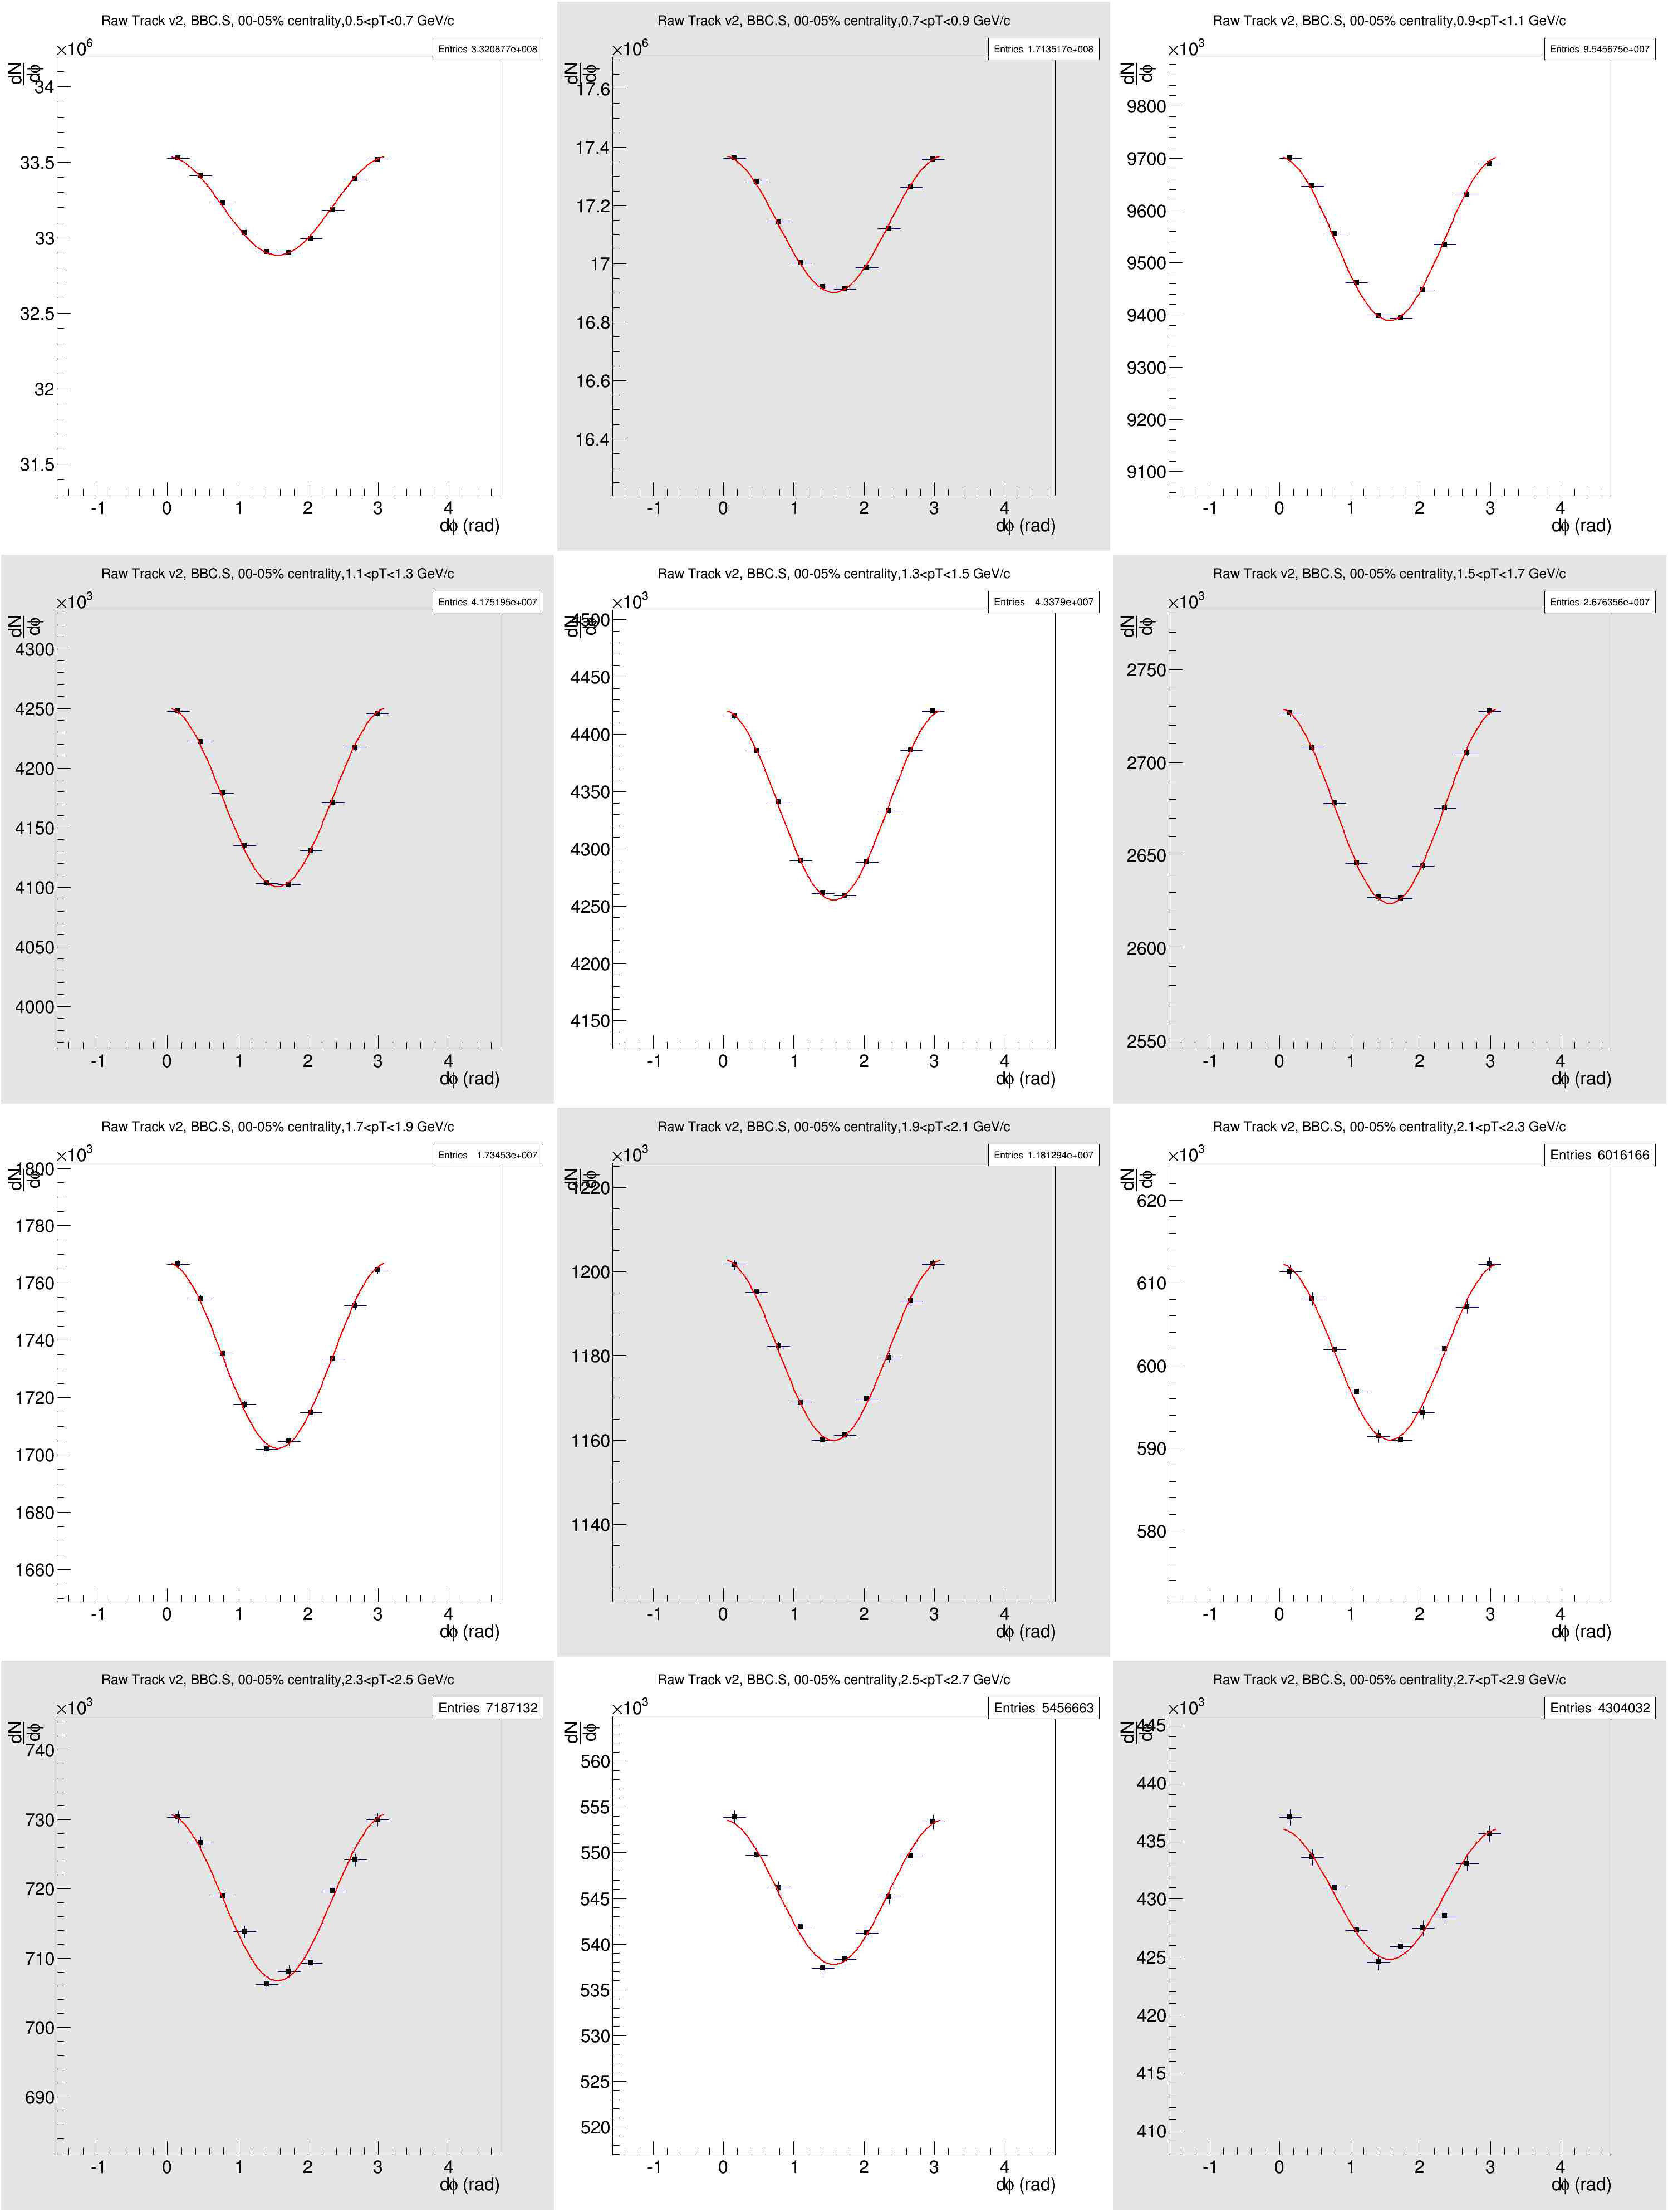
\includegraphics[width=1\textwidth]{chargedtrackv2/htrkdphi2bbcs_0.jpg}
    \rule{35em}{0.5pt}
  \caption[$\frac{d^N}{d\phi}$ vs $d\phi$, 0-5\% centrality.]{$\frac{d^N}{d\phi}$ vs $d\phi$, 0-5\% centrality, each plot represents a 0.2 GeV slice in transverse momentum space.}
  \label{fig:Ndphicent0}
\end{figure}

\begin{figure}[htbp!]
  \centering
    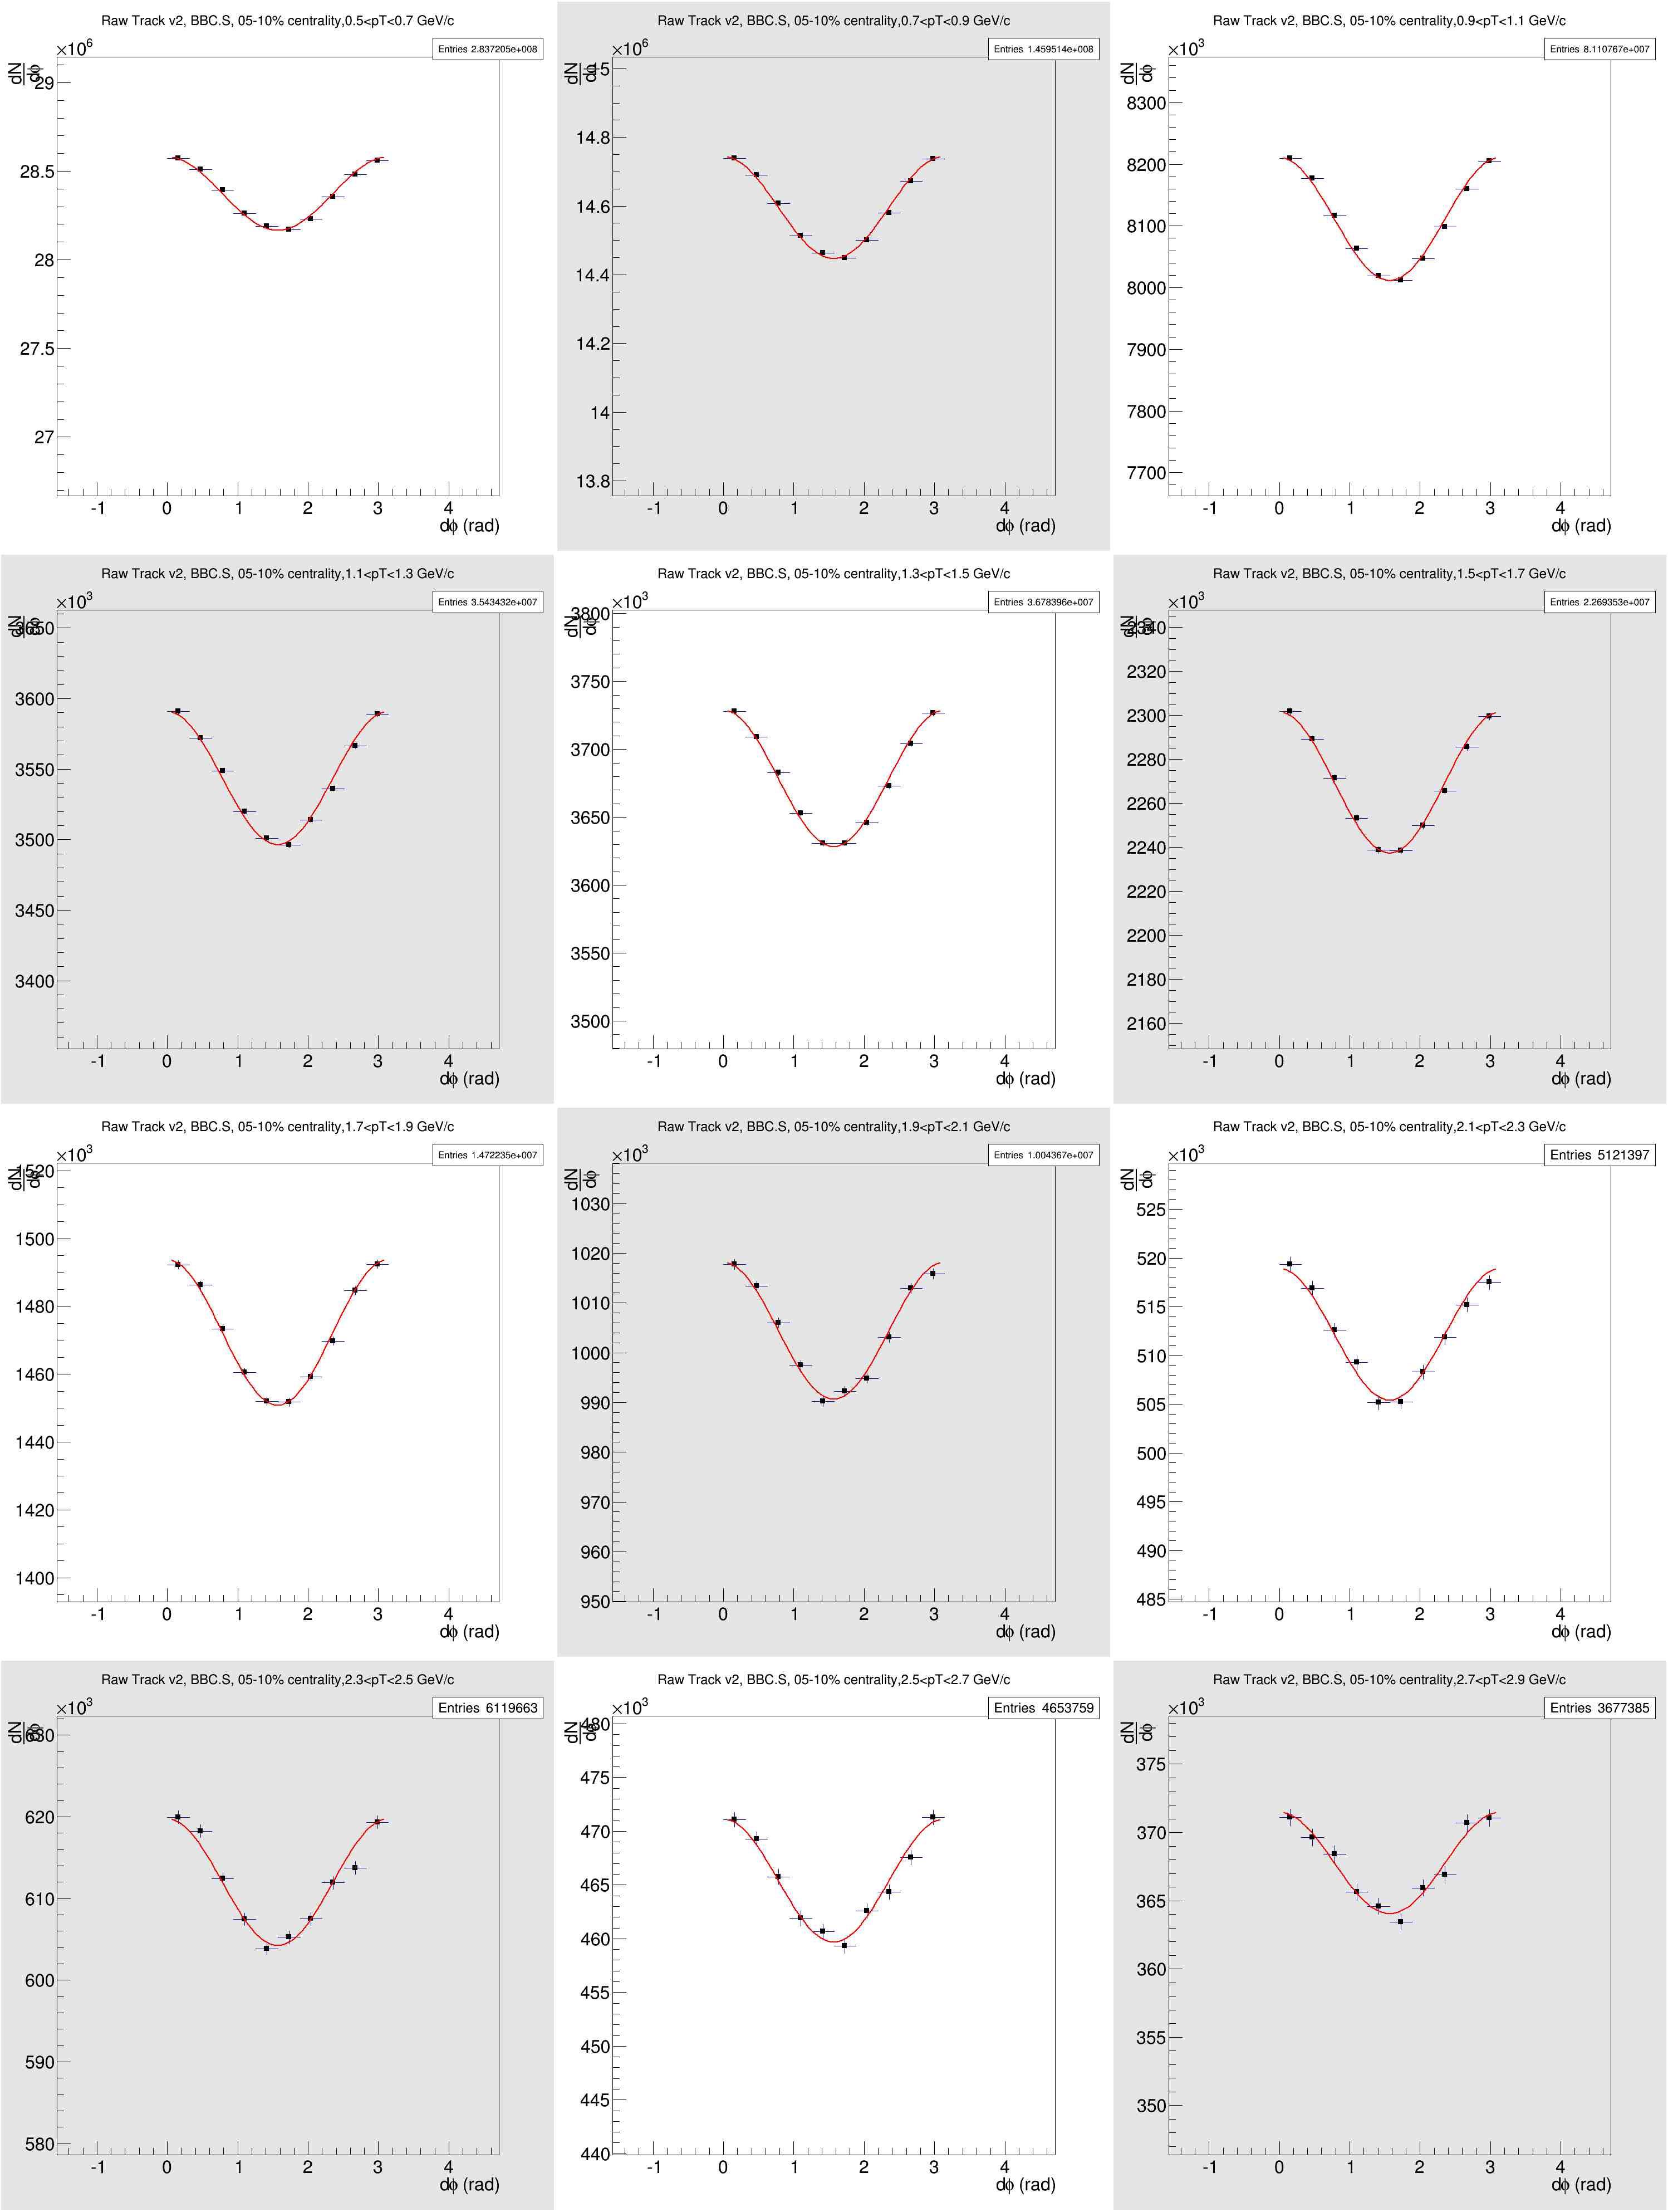
\includegraphics[width=1\textwidth]{chargedtrackv2/htrkdphi2bbcs_1.jpg}
    \rule{35em}{0.5pt}
  \caption[$\frac{d^N}{d\phi}$ vs $d\phi$, 5-10\% centrality.]{$\frac{d^N}{d\phi}$ vs $d\phi$, 5-10\% centrality, each plot represents a 0.2 GeV slice in transverse momentum space.}
  \label{fig:Ndphicent1}
\end{figure}
\begin{figure}[htbp!]
  \centering
    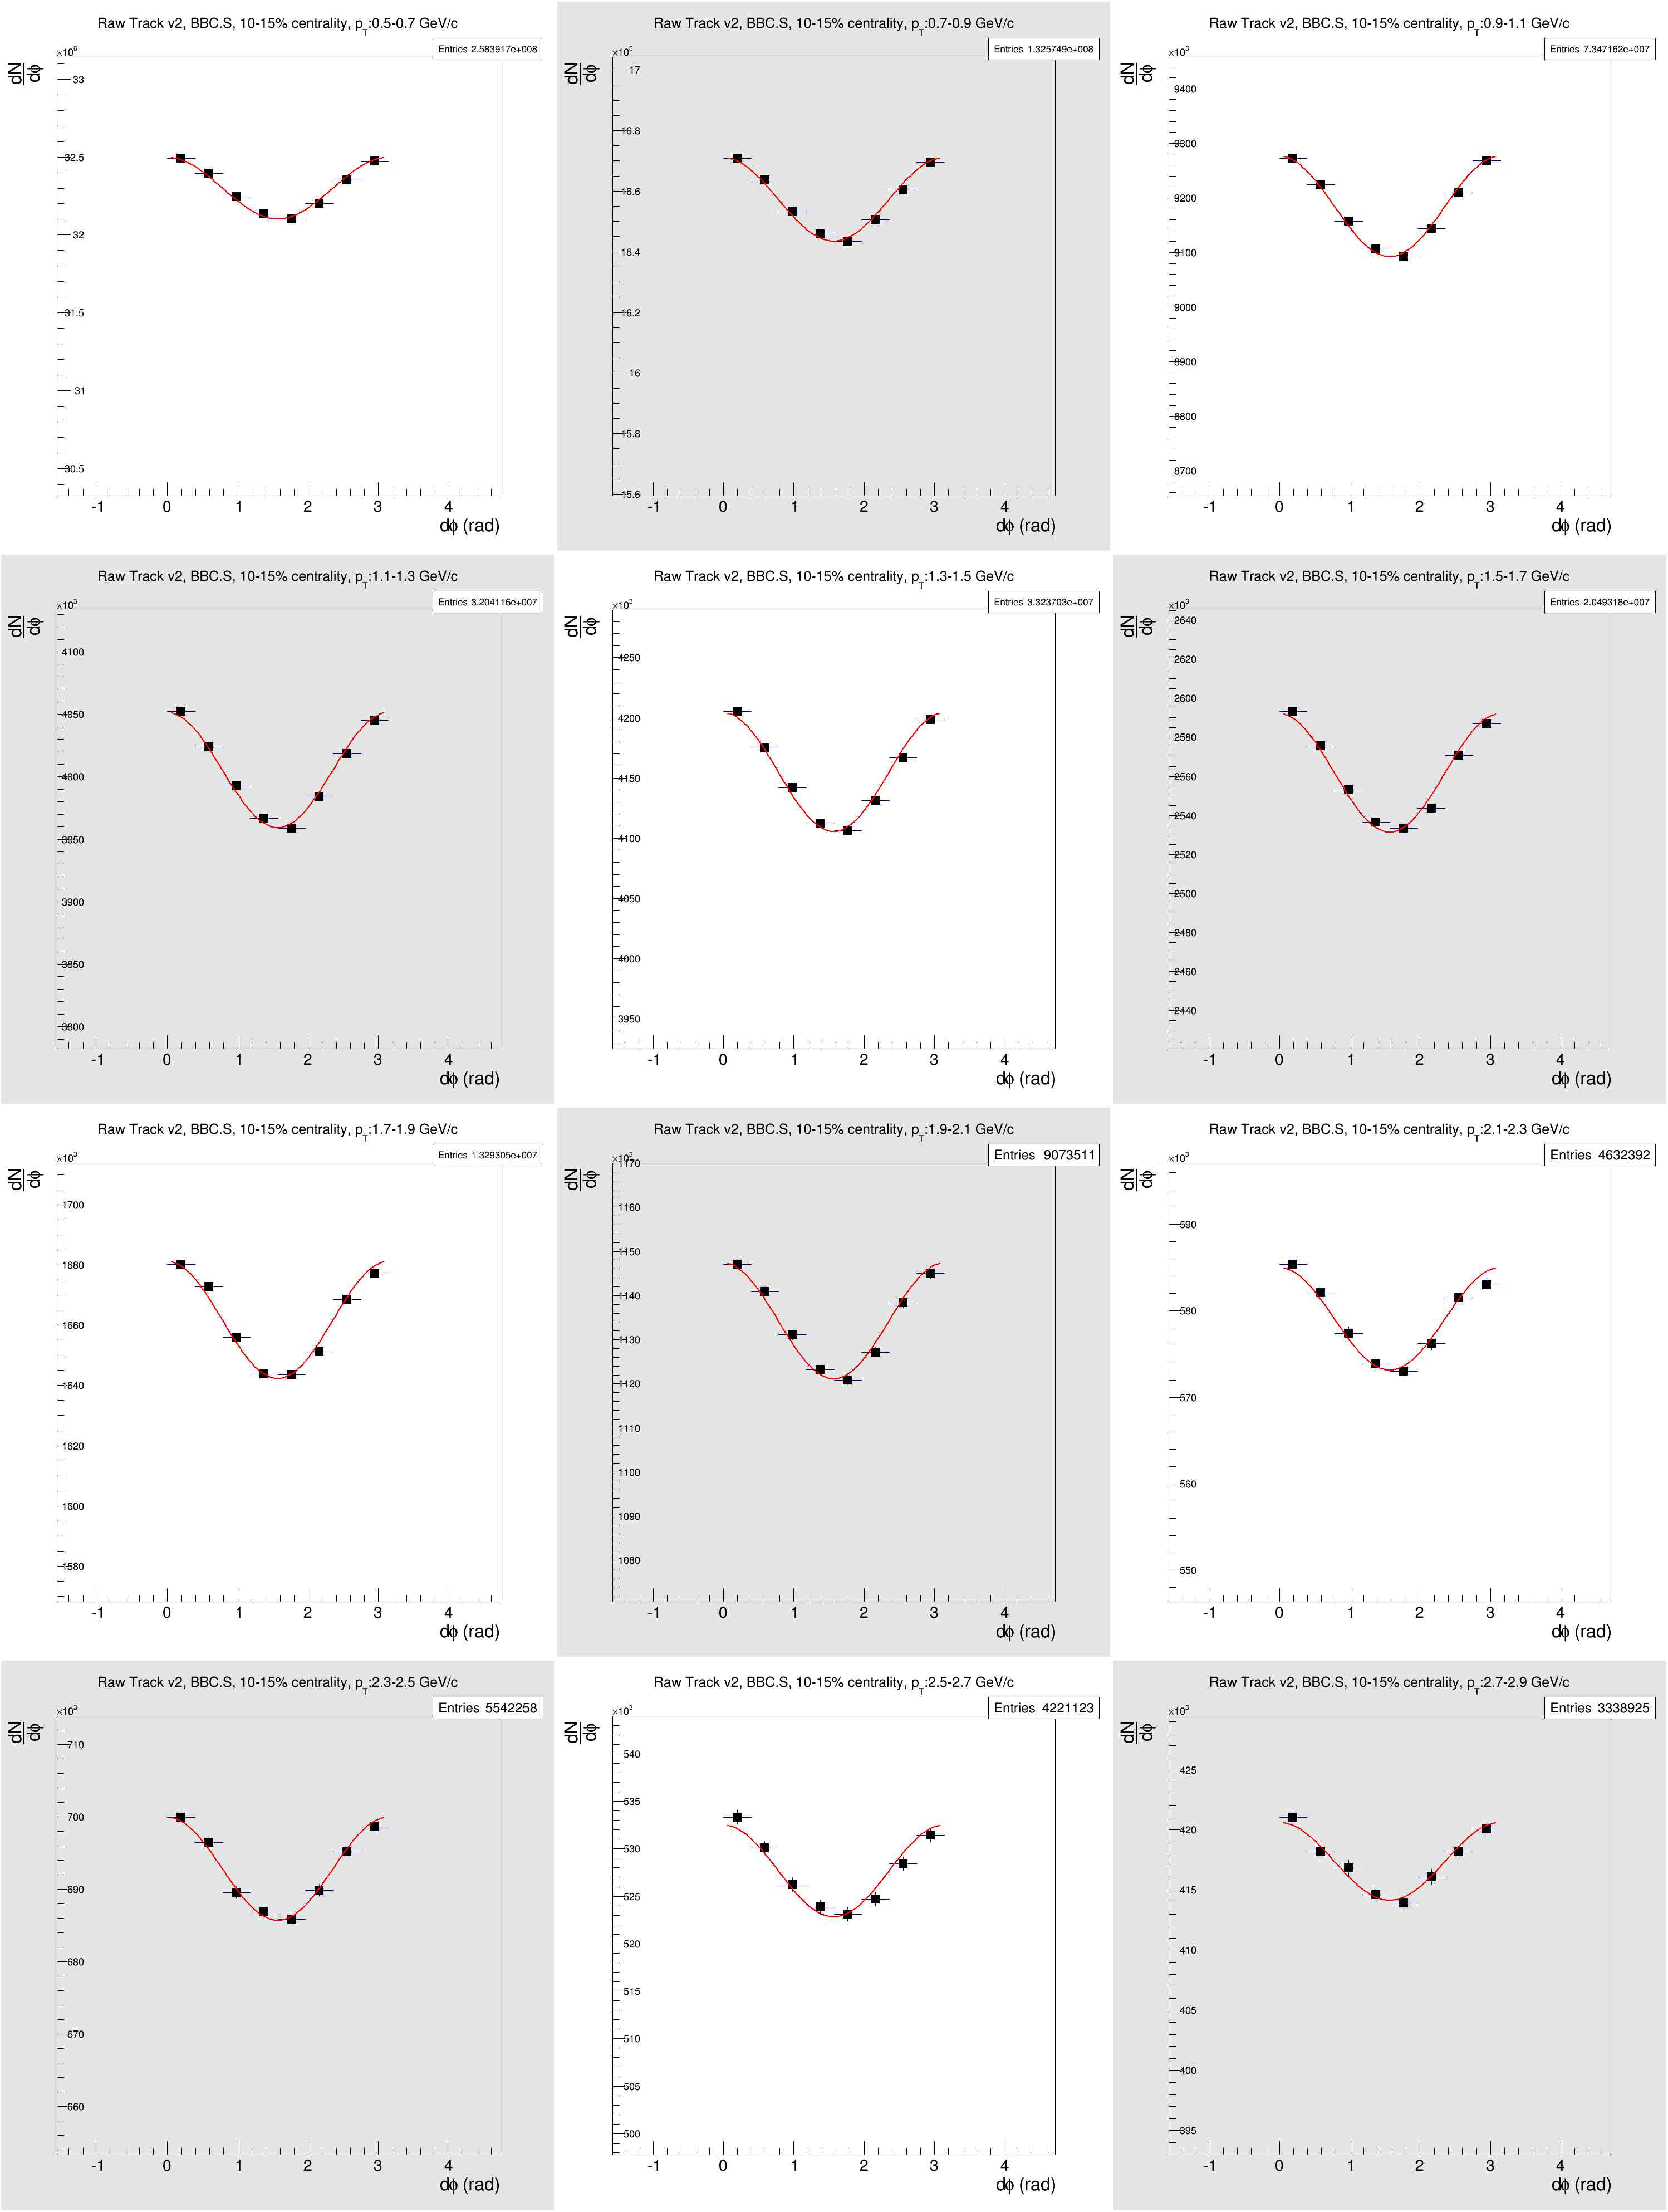
\includegraphics[width=1\textwidth]{chargedtrackv2/htrkdphi2bbcs_2.jpg}
    \rule{35em}{0.5pt}
  \caption[$\frac{d^N}{d\phi}$ vs $d\phi$, 10-15\% centrality.]{$\frac{d^N}{d\phi}$ vs $d\phi$, 10-15\% centrality, each plot represents a 0.2 GeV slice in transverse momentum space.}
  \label{fig:Ndphicent2}
\end{figure}
\begin{figure}[htbp!]
  \centering
    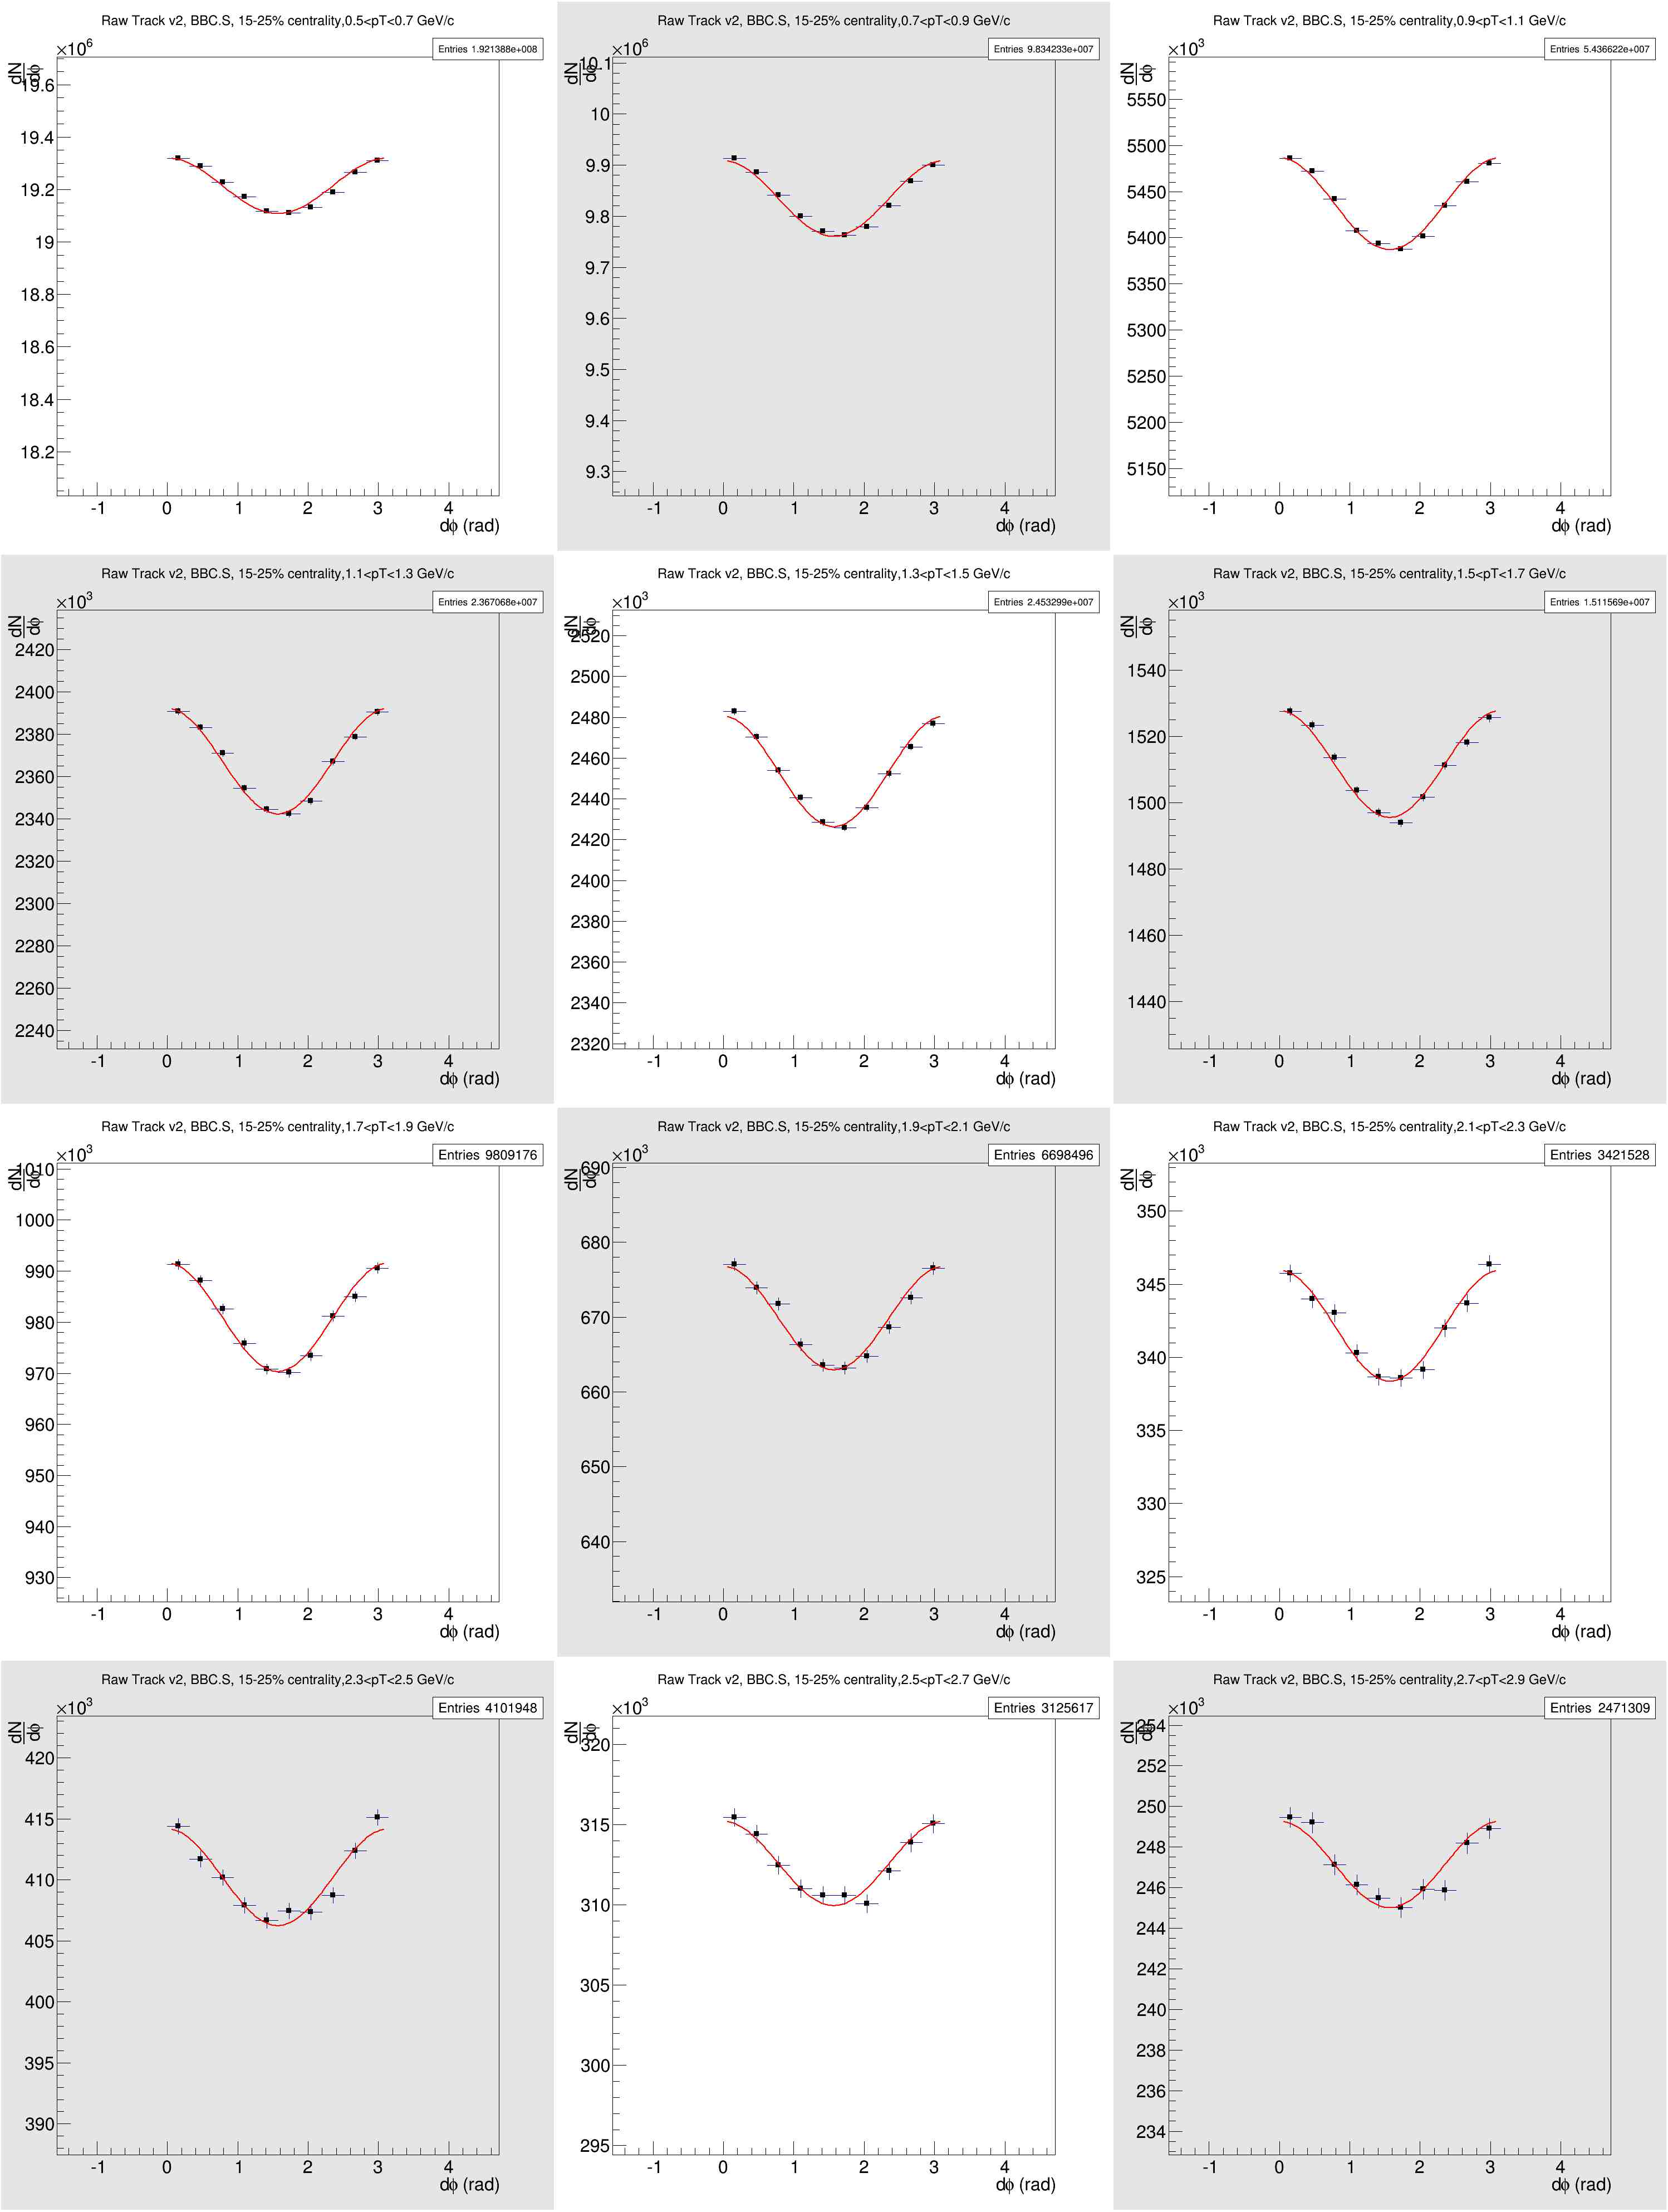
\includegraphics[width=1\textwidth]{chargedtrackv2/htrkdphi2bbcs_3.jpg}
    \rule{35em}{0.5pt}
  \caption[$\frac{d^N}{d\phi}$ vs $d\phi$, 15-25\% centrality.]{$\frac{d^N}{d\phi}$ vs $d\phi$, 15-25\% centrality, each plot represents a 0.2 GeV slice in transverse momentum space.}
  \label{fig:Ndphicent3}
\end{figure}

Which after fitting with the aforementioned cosine function gives the elliptic flow measurements vs centrality shown in figure \ref{fig:alltrackv2}.

\begin{figure}[htbp!]
  \centering
    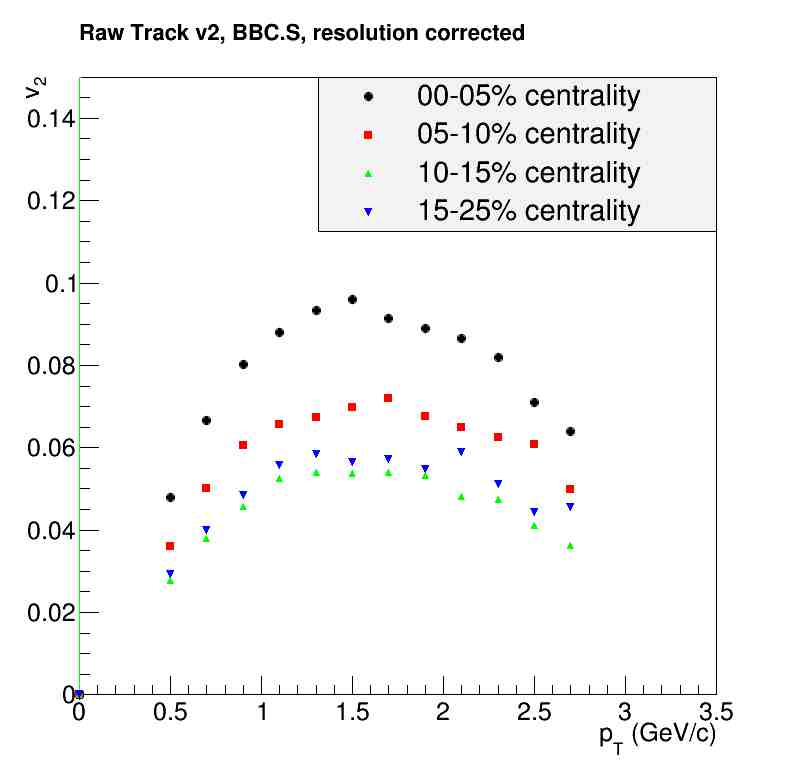
\includegraphics[width=0.7\textwidth]{chargedtrackv2/rawtrackv2_bbcNS.jpg}
    \rule{35em}{0.5pt}
  \caption[Charged track elliptic flow,$\sqrt{s_{NN}}=$200 GeV d+Au collisions]{Charged track elliptic flow,$\sqrt{s_{NN}}=$200 GeV d+Au collisions}
  \label{fig:alltrackv2}
\end{figure}
\section{Separating Particle Signals}
Following the flattening of the event plane and checking for calibration of the TOF detector, we can plot a 2-d histogram of $p_T$ vs $m^2$ following the method described in section \ref{sect:pidmethod} to identify the species of charged track hits in the TOF. In order to do a statistical analysis, these 2-d histograms will need to be ``sliced'' into a series of 1-d histograms in small bins of $p_T$ which will give a 3-peak histogram showing the signatures of the pion, kaon, and proton which are Gaussian in shape. The widths and heights of these particle peaks will change and overlap in various ways over the variance of $p_t$, because of this I will divide the $p_T$ range into three ranges which will be analyzed with different methods.  
\subsection{Single Gaussians}
For $p_T< 1.3$, there is enough separation between the pion, kaon, and proton signals to fit each particle peak with a single Gaussian. This will take the form:
\begin{equation}
f(x) = \frac{N_0}{\sqrt{2\pi \sigma^2}} e^{-\frac{(x-\mu)^2}{2\sigma^{2}}},
\end{equation}
where $\sigma$ is the width of the identified particle peak, $\mu$ is the location of the peak's mean along the x-axis, and $N_0$ is the height of the peak.




\subsection{Gaussian Mixing}
\subsection{ACC as a Pion Discriminator}
\section{Yield vs Event Plane}
\section{Identified Particle $v_{2}$}

\pagebreak
\pagebreak
